\documentclass[final,5p,times,twocolumn]{elsarticle}
\usepackage{amsmath,amssymb,bm,mathtools}
\usepackage{booktabs,array,tabularx,graphicx,microtype}
\newcolumntype{Y}{>{\raggedright\arraybackslash}X}
\usepackage[dvipsnames,table]{xcolor}
\usepackage{enumitem}
\usepackage[hidelinks]{hyperref}
\usepackage[nameinlink,capitalize]{cleveref}
\definecolor{spptBlue}{HTML}{356E9F}
\definecolor{spptGreen}{HTML}{3B8A68}
\definecolor{spptOrange}{HTML}{D8872A}
\definecolor{spptRed}{HTML}{B84A3A}
\definecolor{spptLight}{HTML}{EDF2F5}
\newcommand{\Rmap}{\mathcal R}
\newcommand{\Proj}{\Pi}
\newcommand{\Adm}{\operatorname{Adm}}
\newcommand{\Valid}{\operatorname{Valid}}
\newcommand{\WP}{\operatorname{WP}}
\newcommand{\Attrib}{\operatorname{Attrib}}
\journal{Applied Energy}
\setlength{\parskip}{0pt}
\setlength{\textfloatsep}{8pt plus 2pt minus 2pt}
\setlength{\floatsep}{7pt plus 2pt minus 2pt}
\setlength{\intextsep}{7pt plus 2pt minus 2pt}

\begin{document}
\begin{frontmatter}
\title{Trustworthy AI-Assisted Modeling and Analysis of
Converter-Dominated Hybrid AC/DC Distribution Systems}
\author[xjtu]{High-Resilience Power \& Energy Systems Group}
\affiliation[xjtu]{organization={School of Electrical Engineering,
Xi'an Jiaotong University},city={Xi'an},country={China}}
\begin{abstract}
Converter-dominated hybrid AC/DC distribution systems are increasingly used to
integrate distributed generation, energy storage, electric vehicles, DC loads,
and networked microgrids. Their analysis frequently requires the conversion of
heterogeneous engineering data and is therefore a natural application for
artificial intelligence (AI). However, a successfully converted model or a
converged power flow does not ensure that the resulting equations retain the
authored network topology, converter controls, or device identities. This study
develops a trustworthy AI-assisted modeling framework based on
semantics-preserving projection from detailed engineering models to a canonical
hybrid AC/DC nodal representation. The method establishes explicit
correspondence between engineering devices and nodal equations, classifies
converter control roles, verifies island reference conditions, and reconstructs
calculated quantities at the device level. AI-proposed modifications are first
applied to an isolated model and are adopted only after the physical,
topological, and numerical conditions have been satisfied. The framework is
evaluated using seven public GridLAB-D distribution feeders with disclosed
AC/DC extensions, 1575 fixed-seed model variants, stress sweeps, three-phase
studies, external-engine comparisons, ablation studies, and constrained AI
modification tests. All 1050 structural faults are detected and localized,
while none of the 175 admissible permutations is rejected. In contrast,
convergence-based screening misses converter-terminal, DC-voltage-support, and
efficiency faults. The results also show that physically plausible but
incorrect setpoints require telemetry or operator confirmation. The proposed
framework provides a verification layer for reliable AI-assisted analysis of
converter-dominated distribution systems.
\end{abstract}
\begin{keyword}
Hybrid AC/DC distribution systems \sep Trustworthy artificial intelligence \sep
Semantics-preserving projection \sep Converter control \sep Model verification \sep
Artificial intelligence
\end{keyword}
\end{frontmatter}

\section{Introduction}\label{sec:introduction}

Distribution networks are evolving from predominantly passive AC feeders into
converter-dominated hybrid AC/DC systems. Photovoltaic generation, battery
storage, electric-vehicle charging, data-center demand, DC microgrids, and
power-electronic transformers all increase the proportion of electricity that
is processed through converters before reaching the final load. Compared with
a conventional radial feeder, the resulting system contains several voltage
levels, bidirectional AC/DC interfaces, and multiple devices capable of
regulating AC voltage, DC voltage, active power, or reactive power. These
features improve controllability but make the relation between an engineering
model and its power-flow equations more difficult to establish.

The operational benefits of hybrid distribution systems have motivated a broad
range of recent studies. Hybrid AC/DC reconstruction has been investigated for
electric-vehicle integration~\cite{yu2023ev}; mobile storage has been coordinated
with outage restoration~\cite{zhang2023outage}; and soft open points have been
used to enlarge renewable dispatchable regions~\cite{li2024dispatchable}.
Related studies consider converter coordination, voltage regulation, network
reconfiguration, and resilience enhancement. Their optimization and control
models generally assume that the network equations have already been assembled
from an internally consistent description. This assumption is reasonable for a
single benchmark prepared by the analyst, but it becomes restrictive when the
same study must combine utility data, public feeder models, manufacturer data,
and automatically generated modifications.

Distribution-system descriptions are inherently heterogeneous. Geographic and
asset databases emphasize location, ownership, and equipment ratings; planning
models emphasize impedances and aggregated demand; and OpenDSS or GridLAB-D
models may include phase connections, controls, protection devices, and
technology-specific objects. The same transformer, switch, converter, or load
can consequently have different names, units, and terminal descriptions in
different data sources. Conversion between these representations is not merely
a syntactic operation. It determines which terminals are retained, how ideal
connections are treated, whether disconnected islands participate in the
calculation, and how a calculated voltage or power is associated with the
original device.

Digital-twin research has highlighted this modeling problem. Learning-based
methods have been used to recover distribution-network structures and operating
patterns~\cite{hua2023dt}, while experimentally validated microgrid studies have
combined physical and virtual representations~\cite{sifat2025dt}. The accuracy
of a digital representation nevertheless depends on more than the agreement of
selected outputs. A model may reproduce a voltage profile while omitting a
converter terminal, assigning an incorrect control role, or aggregating devices
in a manner that prevents the calculated result from being returned to the
physical asset. These errors are especially important in hybrid AC/DC systems,
where the converter role determines both the governing equations and the source
that balances losses.

Artificial intelligence provides a new means of preparing and modifying such
models. Large language models have been applied to building-energy model
generation~\cite{jiang2024eplusllm} and to state-estimation assistance on a
2135-node distribution feeder~\cite{li2026llm}. Reinforcement-learning
applications in AC, DC, and hybrid microgrids are also increasing
~\cite{nasir2025rlreview}. These studies demonstrate that AI can interpret
engineering instructions and select analysis operations. However, language
plausibility and predictive accuracy do not establish that a modified network
remains physically meaningful. A proposed change may refer to a nonexistent
terminal, remove the only DC-voltage-regulating device, or alter an aggregated
quantity whose physical origin is ambiguous. A nonlinear calculation can still
converge after some of these errors because the assembled equations describe a
different, incomplete system.

Existing model checks address only part of this problem. Data validation can
identify invalid identifiers, ranges, and terminal references, but it does not
necessarily determine whether the converter controls close the physical degrees
of freedom of every energized island. Power-flow convergence verifies a root of
the assembled equations, but not the correspondence between those equations and
the authored devices. Model reduction and network equivalencing preserve
selected electrical quantities, yet the reverse association from the reduced
network to the original assets is often outside the formulation. Finally,
general AI reliability tests quantify the quality of generated text or selected
operations, whereas power-system analysis requires an independent physical
assessment of every proposed model modification.

This distinction also separates the present problem from anomaly or outlier
detection. Anomaly detection evaluates whether a value is statistically
unusual relative to measurements or historical data. The present study asks
whether the model is internally consistent even when every numerical value is
plausible. A 10\% load increase may be statistically reasonable and physically
solvable but assigned to the wrong asset; conversely, a missing converter
terminal is invalid regardless of its statistical frequency. The two forms of
assessment are therefore complementary rather than interchangeable.

This paper develops semantics-preserving projection theory (SPPT) as a
device-to-equation and equation-to-device consistency framework for hybrid
AC/DC distribution analysis. Its main contributions are:
\begin{enumerate}[leftmargin=1.7em,itemsep=2pt]
\item A projection from detailed engineering models to a canonical hybrid
AC/DC nodal representation, together with a reverse relation that classifies
calculated quantities as exactly recoverable, bounded approximations,
conservation-based allocations, or unsupported quantities.
\item A converter-role formulation that distinguishes specified variables,
balancing variables, AC angle references, and DC-voltage-regulating devices.
The resulting island conditions are evaluated before the nonlinear calculation.
\item An AI-assisted modification procedure in which the proposed change is
first evaluated on an isolated copy of the engineering model. Only modifications
that satisfy the physical, topological, and device-association conditions are
allowed to replace the accepted model.
\item A distribution-focused evaluation comprising seven public GridLAB-D
feeders with disclosed AC/DC additions, 1575 fixed-seed variants, six structural
fault classes, two plausible parameter-error classes, layer-removal studies,
three-phase stress tests, external-engine comparisons, and 42 AI-assisted
modification cases.
\end{enumerate}
The remainder of this paper is organized as follows. Section~2 defines the
hybrid AC/DC equations and the required consistency conditions. Section~3
develops the projection and device-level reconstruction. Section~4 introduces
converter-role closure and the constrained AI modification procedure.
Sections~5 and 6 present the evaluation design and numerical results,
respectively. Section~7 discusses the scope and limitations, and Section~8
draws the conclusions.

\section{Problem formulation and trust requirements}\label{sec:problem}

\subsection{Rich and canonical hybrid AC/DC models}

Let $S$ contain AC and DC buses, lines, transformers, switches, loads,
distributed resources, storage, VSCs, DC/DC converters, units, phase labels,
controls, and stable device identifiers. The canonical model $C=\Proj(S)$
retains the nodal variables and terminal-equivalent components required by a
declared analysis. Its balanced AC equations are
\begin{align}
P_i^{\rm sp}-\Re\{V_i\sum_jY_{ij}^{*}V_j^{*}\}&=0,\\
Q_i^{\rm sp}-\Im\{V_i\sum_jY_{ij}^{*}V_j^{*}\}&=0,
\label{eq:acbalance}
\end{align}
and the DC equation is
\begin{equation}
P_k^{\rm sp}-v_k\sum_{\ell}G_{k\ell}v_{\ell}=0.
\label{eq:dcbalance}
\end{equation}
A VSC couples the domains through selected control equations and
\begin{equation}
P_{{\rm ac},c}+P_{{\rm dc},c}+P_{{\rm loss},c}=0,
\qquad P_{{\rm loss},c}\ge0.
\label{eq:vscbalance}
\end{equation}
The canonical substrate is deliberately smaller than the engineering model.
This supports robust assembly but obliges the transformation to record what was
expanded, aggregated, merged, approximated, or excluded.

\subsection{Why convergence is not a trust criterion}

A nonlinear solver establishes that an assembled residual is small. It does not
establish that every authored terminal exists, that an efficiency is physical,
that a DC voltage is controlled by a real device, or that a canonical injection
can be attributed to an asset. \Cref{tab:trust-layers} separates these questions.

\begin{table}[t]
\centering
\caption{Evidence layers required before an AI-assisted result is trusted.}
\label{tab:trust-layers}
\small
\begin{tabularx}{\linewidth}{@{}p{0.20\linewidth}p{0.32\linewidth}X@{}}
\toprule
Layer & Question & Representative failure \\
\midrule
Boundary validity & Are identities, units, terminals, and ranges coherent? & A VSC points to a nonexistent AC bus. \\
Physical role & Does each island have required voltage/angle support? & A DC island contains only fixed-power devices. \\
Attribution & Can each result return to a stable engineering identity? & An aggregate has no declared origin. \\
Numerical evidence & Did the solver and an independent equation check agree? & A low internal residual hides assembly error. \\
Intent evidence & Is an admissible value the intended value? & A plausible load is assigned to the wrong asset. \\
\bottomrule
\end{tabularx}
\end{table}

For requested observables $\mathcal O$, admission is
\begin{equation}
\Adm(S,\mathcal O)=\Valid(S)\wedge\WP(\Proj(S))
\wedge\Attrib(\Rmap_S,\mathcal O).
\label{eq:admission}
\end{equation}
The three terms check model boundaries, structural well-posedness from island
roles, and total reconstruction for the requested outputs. Solver and
independent-residual checks follow admission. Intent evidence remains an
external layer based on telemetry, asset records, state estimation, or review.

\section{Semantics-preserving projection and provenance}\label{sec:projection}

\Cref{fig:framework} shows the verification layer. Heterogeneous files and AI
actions populate the rich model; projection constructs canonical equations and
a provenance certificate. AI-generated voltages or flows cannot bypass analysis.

\begin{figure}[t]
\centering
\includegraphics[width=\linewidth]{figures/sppt_mechanism_overview.pdf}
\caption{Mechanism of trustworthy AI-assisted modeling. Rich distribution-system
semantics are projected to a canonical hybrid AC/DC substrate while a provenance
certificate records every transformation. Boundary validity, structural
well-posedness, and attribution remain coupled to the physical equations, so
invalid actions are blocked and accepted observables return to stable device
identities.}
\label{fig:framework}
\end{figure}

The projection is
\begin{equation}
\Proj=\mathcal D\circ\mathcal M\circ\mathcal E\circ\mathcal U,
\label{eq:projection}
\end{equation}
where $\mathcal U$ normalizes units, $\mathcal E$ expands macro devices into
terminal equivalents, $\mathcal M$ contracts declared ideal connections, and
$\mathcal D$ separates de-energized islands. Each stage appends a provenance
relation. Contracting a small nonzero impedance is permitted only when its
threshold and affected observables are certified.

\begin{figure}[t]
\centering
\includegraphics[width=\linewidth]{figures/sppt_mechanism_projection.pdf}
\caption{Semantics-preserving projection and reconstruction. (a) Engineering
converter semantics expand into explicit AC, DC, and coupling equations without
losing terminal origins. (b) Topology normalization records merge classes and
energized scope. (c) The reverse map returns canonical observables to distinct
engineering assets and exposes unsupported quantities.}
\label{fig:projection}
\end{figure}

For exactly preserved observables, the semantic contract is
\begin{equation}
\Rmap_S\!\left(A_C(\Proj(S))\right)=A_S(S).
\label{eq:commuting}
\end{equation}
For reduced models, equality becomes the observable-specific bound
\begin{equation}
\left\|\Rmap_S\!\left(A_C(\Proj(S))\right)-A_S(S)\right\|\le\epsilon_{\Pi}.
\label{eq:approximate-contract}
\end{equation}
Four classes prevent
overclaiming: strongly recoverable quantities; bounded-approximate quantities;
auditable but nonunique allocations for which only origin and conservation are
asserted; and nonrecoverable quantities reported as unsupported.

\section{Converter-role typing and trustworthy AI workflow}\label{sec:workflow}

Converter modes determine which equations constrain the system and which
variables power balance must recover. A $P$--$Q$ converter is grid-following
and contributes no voltage reference; a $V_{dc}$--$Q$ or DC-droop converter
anchors DC potential; and an AC grid-forming role supplies the island angle
reference. The guard uses these physical roles rather than device-class names.

For every energized AC island $\mathcal I_a$ and DC island $\mathcal I_d$,
\begin{equation}
n_{\theta}(\mathcal I_a)=1,\qquad n_v(\mathcal I_d)\ge1,
\label{eq:rolecondition}
\end{equation}
where $n_{\theta}$ counts compatible angle-forming roles and $n_v$ counts
physical DC voltage or droop support. Multiple rigid references require an
explicit coordination law. These conditions are necessary role-closure tests:
they do not guarantee Jacobian nonsingularity away from the operating point,
distance from voltage collapse, or satisfaction of converter limits.

\begin{figure}[t]
\centering
\includegraphics[width=\linewidth]{figures/sppt_mechanism_converter_roles.pdf}
\caption{Converter-role mechanism for structural well-posedness. (a) Compatible
AC angle and DC voltage roles assign reference and balancing quantities.
(b) Fixed-power converter roles alone leave DC-voltage regulation and balancing
power without compatible assignments. (c) The structural incidence between
role equations and variables therefore lacks full rank. (d) Provenance
identifies the responsible converter and supports a role-specific repair before
solving.}
\label{fig:roles}
\end{figure}

The AI assistant may classify an input, extract a parameter with provenance,
select a whitelisted transformation, or propose a repair. Each proposal becomes
a typed action $a=(\text{verb},\text{target},\text{field},\text{value},
\text{authority})$. It is applied to a candidate $S'=a(S)$ and evaluated using
\cref{eq:admission}. Rejection discards $S'$; acceptance commits it and invokes
analysis. Thus a failed proposal cannot contaminate the last admitted model.

\begin{figure}[t]
\centering
\includegraphics[width=\linewidth]{figures/sppt_mechanism_agent.pdf}
\caption{Transactional AI-assisted model editing. (a) Natural-language intent
is converted to a typed, authority-bounded action. (b) The edit is applied only
to an isolated candidate state. (c) A candidate crosses the admission boundary
only after all evidence passes; rejection discards the candidate and preserves
the previously admitted state.}
\label{fig:agent-workflow}
\end{figure}

The authority field separates read-only analysis, model editing, advisory
decisions, and physical control. The present study evaluates the first two.
Passing structural guards neither authorizes autonomous control nor proves that
a plausible value reflects operator intent.

\section{Numerical studies}\label{sec:numerical}
The numerical study treats SPPT as a model-verification method rather than a
new power-flow algorithm. It addresses four questions. \textbf{RQ1} asks whether
public distribution models with different sizes and conversion records can be
formed into reproducible hybrid AC/DC cases. \textbf{RQ2} determines which
structural and converter-role faults are missed when convergence is used as the
only acceptance criterion. \textbf{RQ3} evaluates whether calculated quantities
and rejected modifications can be associated with their engineering devices
and fields. \textbf{RQ4} identifies the remaining uncertainty when AI-proposed
modifications or external data contain plausible but incorrect values.

\subsection{Public distribution cases and reproducible protocol}

The primary corpus consists of seven public GridLAB-D r5643 taxonomy feeders
\cite{gridlabd}, rather than transmission test systems. The conversion procedure
reads each GLM model and retains all warnings and unsupported objects in the
case record. The resulting positive-sequence models range from 32 to 6986 AC buses
and from 21 to 5196 AC branches (\Cref{fig:public-feeders}). All seven imports
have zero omitted objects; the 4--61 warnings are retained as evidence of the
conversion range rather than silently discarded. The procedure supports the
balanced steady-state quantities used in the main campaign and does not claim
complete preservation of unbalanced phase controls, protection functions, or
every technology-specific GridLAB-D object.

Each imported feeder receives the same fully specified, deterministic
two-terminal DC overlay. A PQ-controlled VSC is connected to the AC bus carrying
the largest imported active load and a VDC-Q converter to the imported source
bus. The converters connect two DC buses through one line with
$r_{\rm dc}=0.02$~p.u.; the voltage-forming converter regulates
$V_{\rm dc}=1.02$~p.u.; both converters use $\eta=0.99$. The PQ transfer is
\begin{equation}
 P_{\rm PQ}=\operatorname{clamp}
 \left(0.02P_{\rm load,total},\,0.001S_{\rm base},\,0.05S_{\rm base}\right).
 \label{eq:public-overlay}
\end{equation}
Thus the hybridization is reproducible from public data and the stated rule;
it is not calibrated to an undisclosed utility network. The case definition
records the public source, converted network size, retained warnings, AC and DC
terminals, converter controls, setpoints, efficiency, and DC branch for every
case. \Cref{tab:public-cases} summarizes the seven systems.

\begin{figure*}[t]
  \centering
  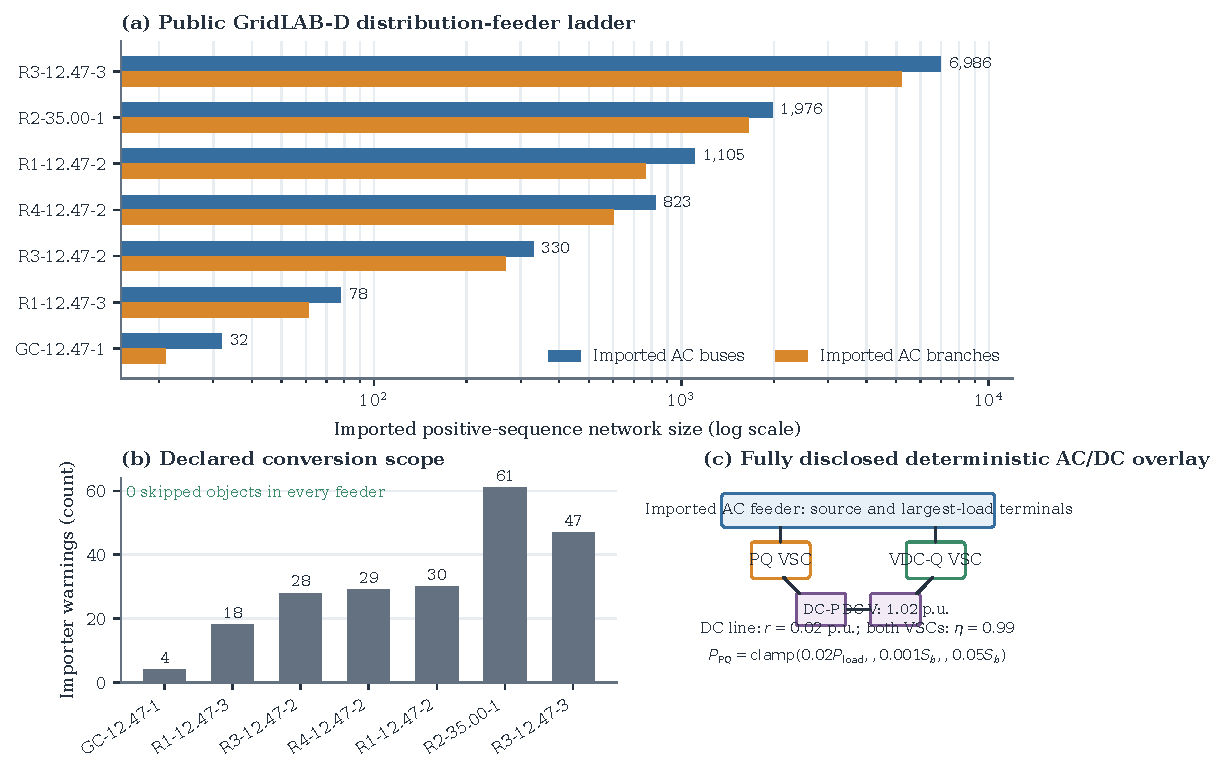
\includegraphics[width=\textwidth]{figures/sppt_public_feeder_variants.pdf}
  \caption{Public distribution benchmark and deterministic hybridization.
  (a) Imported AC buses and branches on a logarithmic scale; (b) retained
  importer warnings and zero skipped objects; and (c) the disclosed AC/DC
  overlay applied identically to each feeder.}
  \label{fig:public-feeders}
\end{figure*}

\begin{table*}[t]
\centering
\caption{Public distribution feeders and disclosed hybrid AC/DC extensions.}
\label{tab:public-cases}
\small
\begin{tabular}{@{}lrrrrrrr@{}}
\toprule
System & AC buses & AC branches & Conversion warnings & Omitted objects & PQ-VSC AC bus & $P_{\rm PQ}$ (MW) & $V_{dc}$ (p.u.)\\
\midrule
GC-12.47-1-ACDC & 32 & 21 & 4 & 0 & 1 & 0.1065 & 1.02\\
R1-12.47-3-ACDC & 78 & 61 & 18 & 0 & 76 & 0.0268 & 1.02\\
R3-12.47-2-ACDC & 330 & 267 & 28 & 0 & 57 & 0.0873 & 1.02\\
R4-12.47-2-ACDC & 823 & 601 & 29 & 0 & 332 & 0.0479 & 1.02\\
R1-12.47-2-ACDC & 1105 & 763 & 30 & 0 & 2 & 0.0564 & 1.02\\
R2-35.00-1-ACDC & 1976 & 1656 & 61 & 0 & 383 & 0.2056 & 1.02\\
R3-12.47-3-ACDC & 6986 & 5196 & 47 & 0 & 108 & 0.1613 & 1.02\\
\bottomrule
\end{tabular}
\end{table*}

The prespecified generator uses MT19937-64 with seed 20260818 and 25 repetitions
per case and perturbation class. It produces
$7\times9\times25=1575$ rows: 175 valid component-order permutations, 1050
structural faults, and 350 plausible intention errors. The six structural
classes remove a VSC AC terminal, remove a VSC DC terminal, remove the AC angle
reference, remove physical DC-voltage support, set converter efficiency above
unity, or duplicate an AC-bus identity. The two intention-error classes multiply
one imported load by a factor in $[0.70,1.30]$ or apply a nonzero signed
perturbation to the in-service PQ-VSC active-power setpoint. No failed,
nonconverged, or inconvenient sample is removed.

Five comparative assessments are recorded: model-integrity checks,
convergence-based screening, model integrity followed by convergence, complete
SPPT assessment, and SPPT followed by an independently formed primitive-equation
residual. A convergence-based rejection means nonconvergence, a nonfinite
residual, or a residual greater than $10^{-6}$.
Detection means refusing an injected structural fault; localization additionally
requires the diagnostic to identify its component and field, or its affected
AC/DC island reference. The 95\% intervals use the Wilson score interval. To
bound computational cost without selecting outcomes, convergence-only
trials are fixed to the 32-, 78-, and 330-bus cases, whereas physical-impact
solves are fixed to the 32-, 78-, 330-, and 823-bus cases. Every case remains in
model-integrity, projection, device-association, and complete-SPPT tests.

\begin{table*}[t]
\centering
\caption{Perturbation classes used in the 1575-case campaign.}
\label{tab:fault-classes}
\small
\begin{tabularx}{\textwidth}{@{}p{0.24\textwidth}p{0.25\textwidth}p{0.23\textwidth}X@{}}
\toprule
Class & Modification & Physical consequence & Principal assessment\\
\midrule
Valid permutation & Reorder component storage without changing identities or data & Same physical model and results & False-rejection control\\
Missing VSC AC terminal & Replace the AC terminal by a nonexistent bus & Incomplete converter connection & Model integrity\\
Missing VSC DC terminal & Replace the DC terminal by a nonexistent bus & Incomplete AC/DC coupling & Model integrity\\
Missing AC reference & Remove the only compatible AC angle-forming role & AC island equations not closed & Island-role assessment\\
Missing DC support & Change the $V_{dc}$-regulating converter to fixed $P$--$Q$ control & DC voltage and balancing power lack compatible roles & Converter-role assessment\\
Invalid efficiency & Set $\eta_c>1$ & Artificial conversion gain & Physical range assessment\\
Duplicate AC identity & Assign one stable AC-bus identity to two devices & Ambiguous topology and result association & Identity and device association\\
Plausible load error & Multiply one load by a value in $[0.70,1.30]$ & Solvable but potentially incorrect operating state & External operating evidence\\
Plausible VSC error & Apply a nonzero signed change to $P_{\rm PQ}$ & Solvable but potentially incorrect power transfer & External operating evidence\\
\bottomrule
\end{tabularx}
\end{table*}

For fault class $f$, the detection and localization rates are
\begin{equation}
 r_f^{\rm det}=\frac{N_f^{\rm det}}{N_f},\qquad
 r_f^{\rm loc}=\frac{N_f^{\rm loc}}{N_f}.
 \label{eq:detection-metrics}
\end{equation}
The Wilson interval is used instead of the normal approximation because several
observed rates are zero or unity. For $k$ detections in $n$ samples and
$z=1.96$, the interval center and half-width are
\begin{align}
 c&=\frac{k/n+z^2/(2n)}{1+z^2/n},\\
 h&=\frac{z}{1+z^2/n}
 \sqrt{\frac{(k/n)(1-k/n)}{n}+\frac{z^2}{4n^2}}.
 \label{eq:wilson}
\end{align}
The reported 95\% interval is $[c-h,c+h]$. The valid permutations provide the
corresponding false-rejection estimate.

\section{Results and analysis}\label{sec:results}

\subsection{Structural safety benefit and solver blind spots}

The full SPPT chain detects and localizes all 1050 structural faults. Pooling the
six classes gives 1.000 detection with a 95\% Wilson interval
$[0.9964,1.000]$. It rejects none of the 175 valid permutations, corresponding
to a false-reject estimate of zero and a 95\% upper bound of 0.0215. These
controls are important: perfect fault detection alone could otherwise be
obtained by rejecting every model.

\Cref{fig:structural-detection} separates the assessment layers. Model-integrity
checks detect terminal, efficiency, identity, and AC-reference faults, but
misses all 175 missing-DC-support cases. Converter-role typing closes precisely
this gap. Convergence-based screening is weaker: among the three in-scope feeders it
misses all dangling VSC terminals, all missing DC support, and all invalid
efficiencies; it rejects the missing AC reference and only 3 of 75 duplicate
identities. Hence numerical convergence establishes a root of the assembled
equations, not completeness or physical meaning of the authored model.

\begin{figure*}[t]
  \centering
  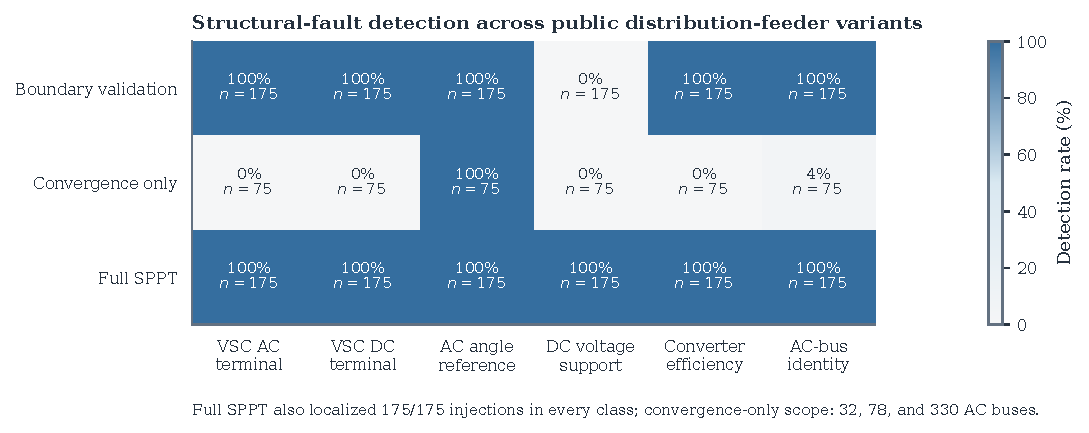
\includegraphics[width=\textwidth]{figures/sppt_structural_detection.pdf}
  \caption{Detection rate by fault class and assessment level. Model-integrity
  and complete-SPPT results use 175 samples per class across all seven public
  feeder variants. Convergence-based results use 75 samples per class on the
  prespecified 32-, 78-, and 330-bus range. Complete SPPT also localizes all
  175 instances in every structural class.}
  \label{fig:structural-detection}
\end{figure*}

The comparison is also a functional ablation. Removing role typing from the
full chain recreates the 0/175 missing-DC-support result of model-integrity
checking. Removing those checks and retaining only the nonlinear solution recreates four complete
blind spots plus the 4\% duplicate-identity rejection rate. Adding an
independent residual does not change structural counts because those samples
are rejected before solution; its distinct purpose is to check an admitted
state against equations independent of the primary analysis path.

\begin{table*}[t]
\centering
\caption{Structural-fault detection obtained by model-integrity checks,
convergence-based screening, and complete SPPT assessment.}
\label{tab:detection-results}
\footnotesize
\begin{tabularx}{\textwidth}{@{}Xrrrrrr@{}}
\toprule
Fault class & Samples & Integrity detected & Convergence samples & Convergence detected & SPPT detected & SPPT localized\\
\midrule
Missing VSC AC terminal & 175 & 175 & 75 & 0 & 175 & 175\\
Missing VSC DC terminal & 175 & 175 & 75 & 0 & 175 & 175\\
Missing AC reference & 175 & 175 & 75 & 75 & 175 & 175\\
Missing DC support & 175 & 0 & 75 & 0 & 175 & 175\\
Invalid converter efficiency & 175 & 175 & 75 & 0 & 175 & 175\\
Duplicate AC identity & 175 & 175 & 75 & 3 & 175 & 175\\
\bottomrule
\end{tabularx}
\end{table*}

The pooled result is not produced by one small feeder. Each of the seven
systems contributes 225 variants: 25 valid permutations, 150 structural
faults, and 50 plausible parameter modifications. \Cref{tab:feeder-results}
reports the feeder-wise outcomes. All structural faults are detected and
localized on every network, including the 6986-bus case, and all valid
permutations are accepted. The 200 parameter-impact calculations are confined
by the prespecified scope to the four feeders up to 823 buses. Their response
is not monotonic in bus count: the largest branch-power deviation occurs on
the 32-bus feeder, whereas the largest voltage deviation occurs on the
823-bus feeder. This observation supports the use of heterogeneous public
feeders rather than interpreting system size as a proxy for physical
sensitivity.

\begin{table*}[t]
\centering
\caption{Feeder-wise outcomes of the fixed-seed assessment campaign.}
\label{tab:feeder-results}
\footnotesize
\begin{tabularx}{\textwidth}{@{}lrrrrrrX@{}}
\toprule
Public hybrid feeder & AC buses & Total variants & Structural detected/localized & Valid accepted & Impact calculations & Max. $|\Delta V_{ac}|$ (p.u.) & Max. $|\Delta P_{branch}|$ (MW) \\
\midrule
GC-12.47-1 & 32 & 225 & 150/150 & 25/25 & 50/50 & $4.02\!\times\!10^{-4}$ & 0.526 \\
R1-12.47-3 & 78 & 225 & 150/150 & 25/25 & 50/50 & $1.70\!\times\!10^{-3}$ & 0.0305 \\
R3-12.47-2 & 330 & 225 & 150/150 & 25/25 & 50/50 & $2.82\!\times\!10^{-3}$ & 0.169 \\
R4-12.47-2 & 823 & 225 & 150/150 & 25/25 & 50/50 & $4.24\!\times\!10^{-3}$ & 0.0297 \\
R1-12.47-2 & 1105 & 225 & 150/150 & 25/25 & -- & -- & -- \\
R2-35.00-1 & 1976 & 225 & 150/150 & 25/25 & -- & -- & -- \\
R3-12.47-3 & 6986 & 225 & 150/150 & 25/25 & -- & -- & -- \\
\midrule
Total & -- & 1575 & 1050/1050 & 175/175 & 200/200 & $4.24\!\times\!10^{-3}$ & 0.526 \\
\bottomrule
\end{tabularx}
\end{table*}

The different failure patterns explain why the assessment levels are not
interchangeable. A missing terminal can disappear from the equation set and is
therefore invisible to convergence. An efficiency above unity can still define
a smooth set of equations although it violates energy conservation. Missing DC
support is topologically valid but fails the role-closure test. Duplicate
identities are occasionally exposed by numerical singularity, but the 3/75
rejection rate shows that convergence is an unreliable identity check. In
contrast, the missing AC reference directly creates a numerical degree of
freedom and is detected by both the physical assessment and the nonlinear
calculation.

\subsection{Device association and the intent-error boundary}

Every valid permutation satisfies the requested device association for AC-bus
voltage, DC-bus voltage, and converter transfer. The projection is therefore
invariant to component-storage order while the results remain addressed by
stable engineering identities. For the rejected modifications, all 1050
diagnoses return to the modified device and field or to the affected island
reference. The localization result is not inferred from the perturbation label;
it is obtained from the same forward and reverse relations used for an
unmodified case.

Additional round-trip evaluations distinguish intensive and extensive
quantities. A bus voltage is broadcast to all buses in the corresponding ideal
merge class. Branch and device powers are returned according to their physical
origin or a declared participation rule whose coefficients sum to unity.
Unsupported internal quantities are reported as unavailable rather than being
assigned an artificial value. The fault-localization experiment therefore
examines engineering input diagnosis, whereas the round-trip evaluation
examines reconstruction of calculated results.

Neither SPPT nor an outlier detector can infer operator intent from a single
self-consistent model. All 350 plausible load and VSC-setpoint edits preserve
references, limits, identities, and equation consistency, so all structural
chains admit them. Their physical consequences are nevertheless nonzero
(\Cref{fig:intent-impact}). On the four feeder variants with impact solves, a
load edit gives median/95th-percentile/maximum AC-voltage deviations of
$3.089\times10^{-4}$/$1.652\times10^{-3}$/$4.239\times10^{-3}$~p.u. and branch
active-power deviations of 0.00524/0.427/0.526~MW. A VSC-setpoint edit gives
AC-voltage deviations of $1.821\times10^{-4}$/$1.828\times10^{-3}$/$1.916\times10^{-3}$~p.u.,
DC-voltage deviations of $3.706\times10^{-5}$/$5.844\times10^{-5}$/$6.322\times10^{-5}$~p.u.,
branch-flow deviations of 0.0192/0.0300/0.0320~MW, and converter-transfer
deviations of 0.0189/0.0298/0.0322~MW. Here the empirical 95th percentile is the
nearest observed order statistic. The zero DC/VSC response to load edits follows
from the fixed PQ transfer in \Cref{eq:public-overlay}; it is not missing data.

\begin{figure*}[t]
  \centering
  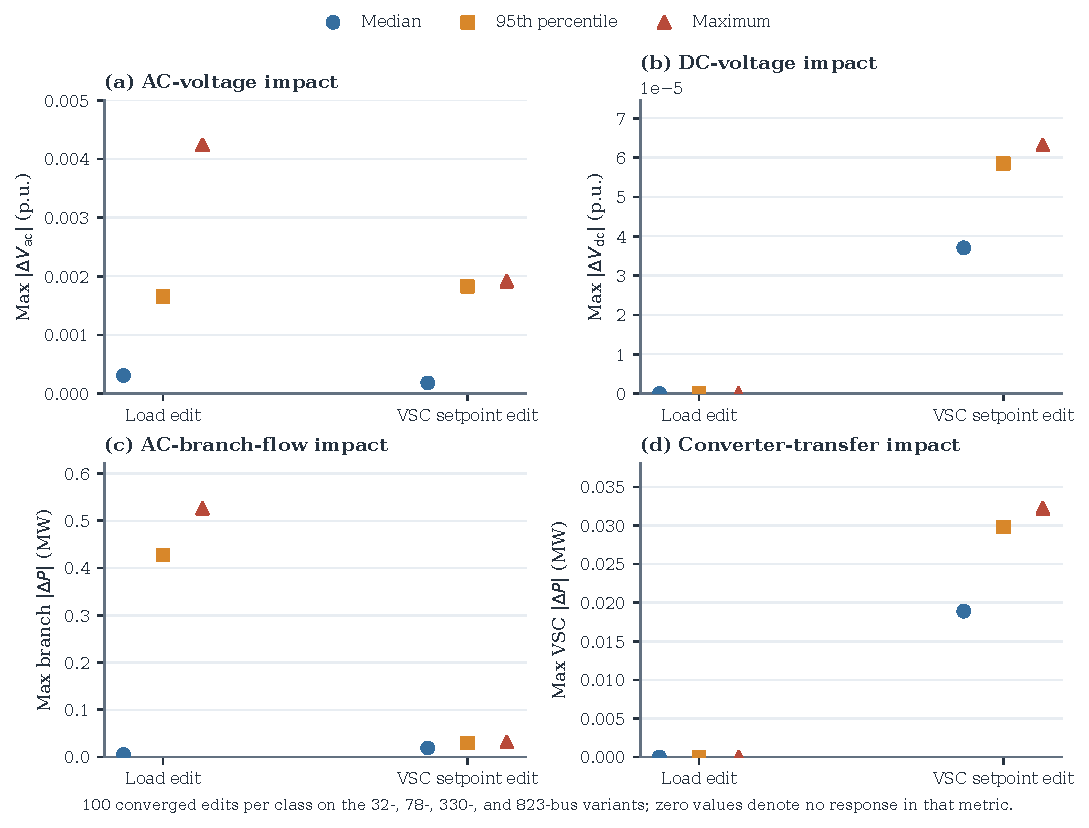
\includegraphics[width=\textwidth]{figures/sppt_intent_error_impacts.pdf}
  \caption{Physical consequences of structurally admissible but incorrect
  values, shown as median, empirical 95th percentile, and maximum over 100
  converged edits per class. Separate panels preserve the units of AC voltage,
  DC voltage, AC-branch power, and VSC transfer.}
  \label{fig:intent-impact}
\end{figure*}

\begin{table*}[t]
\centering
\caption{Physical deviations caused by structurally admissible but incorrect
parameter modifications.}
\label{tab:intent-impact}
\footnotesize
\begin{tabularx}{\textwidth}{@{}Xlrrrrrr@{}}
\toprule
Quantity & Unit & \multicolumn{3}{c}{Load modification} & \multicolumn{3}{c}{VSC-setpoint modification}\\
\cmidrule(lr){3-5}\cmidrule(lr){6-8}
& & Median & 95th percentile & Maximum & Median & 95th percentile & Maximum\\
\midrule
$|\Delta V_{ac}|$ & p.u. & $3.089\!\times\!10^{-4}$ & $1.652\!\times\!10^{-3}$ & $4.239\!\times\!10^{-3}$ & $1.821\!\times\!10^{-4}$ & $1.828\!\times\!10^{-3}$ & $1.916\!\times\!10^{-3}$\\
$|\Delta V_{dc}|$ & p.u. & 0 & 0 & 0 & $3.706\!\times\!10^{-5}$ & $5.844\!\times\!10^{-5}$ & $6.322\!\times\!10^{-5}$\\
$|\Delta P_{branch}|$ & MW & 0.00524 & 0.427 & 0.526 & 0.0192 & 0.0300 & 0.0320\\
$|\Delta P_{VSC}|$ & MW & 0 & 0 & 0 & 0.0189 & 0.0298 & 0.0322\\
\bottomrule
\end{tabularx}
\end{table*}

This experiment marks the method boundary rather than a failure of the
assessment. Parameter traceability, telemetry consistency, state estimation,
operator confirmation, or anomaly detection must provide the external evidence
needed to decide whether a numerically plausible value was intended. SPPT then
checks whether the resulting edited model is structurally valid, well posed,
solvable, and attributable.

\subsection{AI-assisted modification experiment}

The experiment evaluates the isolated-model procedure in
\cref{fig:ai-modification}, rather than treating an AI response as a power-flow
result. Six structured modifications are applied independently to every public
hybrid feeder: a 10\% load increase, an unchanged-model control, two nonexistent
VSC terminal assignments, removal of DC-voltage support, and an above-unity
converter efficiency. Each proposed modification is followed by a valid
unchanged-model assessment, which determines whether a rejected proposal has
altered the accepted model.

All 14 admissible system--modification combinations are accepted and adopted,
while all 28 inadmissible combinations are refused before they can replace the
accepted model (\cref{fig:ai-modification-results}). Every subsequent unchanged-model
assessment is accepted.
End-to-end power flow is prespecified for the 32-, 78-, 330-, and 823-bus
variants: all eight admissible primary modifications and all 24 subsequent
unchanged-model assessments in
that scope converge and return attributed bus voltages. The three larger
feeders remain in physical assessment and model-retention evaluation but are not repeatedly
solved. An unexecuted large-case solve is therefore not counted as either
convergence or failure.

\begin{figure*}[t]
  \centering
  \includegraphics[width=\textwidth]{figures/sppt_agent_public_campaign.pdf}
  \caption{Constrained AI-assisted modification test on seven public hybrid
  distribution feeders. (a) Every admissible modification is adopted and every
  inadmissible modification is refused before replacing the accepted model.
  (b) Refused modifications do not invoke power-flow analysis, and the subsequent
  unchanged-model assessment confirms that the accepted model remains usable.}
  \label{fig:ai-modification-results}
\end{figure*}

\Cref{tab:ai-modifications} gives the exact outcomes behind the figure. The
10\% load change and unchanged-model control are accepted on all seven feeders.
Power flow is then evaluated on the four prespecified feeders, giving eight
converged primary calculations with complete bus-voltage association. Each of
the four physically inadmissible modifications is refused on every feeder and
therefore does not produce a power-flow result. This absence is intentional: a
calculation performed after a known terminal or control-role defect would not
constitute additional evidence. The subsequent unchanged-model assessment is
accepted in all 42 sequences and, where calculation is prescribed, returns the
same engineering identity set as before the proposal.

\begin{table*}[t]
\centering
\caption{Outcomes of the constrained AI-assisted modification experiment.}
\label{tab:ai-modifications}
\footnotesize
\begin{tabularx}{\textwidth}{@{}p{0.24\textwidth}p{0.10\textwidth}p{0.11\textwidth}p{0.12\textwidth}p{0.13\textwidth}X@{}}
\toprule
Proposed modification & Expected decision & Observed decision & Power flow & Following check & Physical basis \\
\midrule
Increase all loads by 10\% & Accept & Accept 7/7 & 4/4 converged & 7/7 accepted & References, roles, and device relations are retained. \\
Leave model unchanged & Accept & Accept 7/7 & 4/4 converged & 7/7 accepted & The engineering and canonical models are identical. \\
Assign nonexistent VSC AC terminal & Refuse & Refuse 7/7 & Not evaluated & 7/7 accepted & The converter has no valid AC connection. \\
Assign nonexistent VSC DC terminal & Refuse & Refuse 7/7 & Not evaluated & 7/7 accepted & The converter has no valid DC connection. \\
Remove DC-voltage support & Refuse & Refuse 7/7 & Not evaluated & 7/7 accepted & The energized DC island lacks a compatible voltage-forming role. \\
Set converter efficiency above unity & Refuse & Refuse 7/7 & Not evaluated & 7/7 accepted & The conversion model introduces nonphysical energy gain. \\
\midrule
Total & -- & 14 accepted; 28 refused & 8/8 converged & 42/42 accepted & -- \\
\bottomrule
\end{tabularx}
\end{table*}

This experiment provides evidence for constrained modification, isolation of
the accepted model, and equation-to-device association. It is not a benchmark
of unrestricted language understanding. An optional five-request local LLM
trial is retained only to show that a language model can populate the structured
engineering modification in \eqref{eq:structured-modification}; its sample size
is not used as statistical evidence of LLM reliability.

\subsection{Three-phase and external-engine scope checks}

The primary campaign uses the imported balanced subset because the public GLM
conversion procedure does not preserve every phase-domain control quantity. A
staged three-phase study therefore exercises three disclosed distribution
variants: a balanced radial feeder, an unbalanced lateral feeder, and an
unbalanced meshed feeder with DER, each coupled to a two-bus DC charger. All
three base points converge. Across load multipliers
$\{0.5,1.0,1.25,1.5,1.75,2.0\}$, the balanced, lateral, and meshed variants
converge at 6/6, 4/6, and 5/6 DC-boundary points, respectively. The failed high
stress points are retained and reported; this staged study demonstrates a
phase-aware modeling range, not equivalence to the positive-sequence
campaign.

External-engine comparisons are similarly qualified. The GridLAB-D conversion
reads and solves the projected AC snapshots of all 24 public taxonomy models;
only seven legacy models can also be evaluated without modification by the
available modern GridLAB-D release, so numerical comparison is restricted to
their 3222 common buses. The OpenDSS study evaluates the official IEEE-13 and
six supplied public EPRI circuits, but only for overlapping three-phase AC
quantities, not for the added DC grid or VSC controls. These comparisons define
the range of common physical quantities rather than treating either external
engine as a universal hybrid AC/DC reference.

\begin{table*}[t]
\centering
\caption{Base-point quantities and stress-study range of the staged three-phase distribution cases.}
\label{tab:three-phase}
\footnotesize
\begin{tabularx}{\textwidth}{@{}lrrrrrrX@{}}
\toprule
Distribution variant & Phase nodes & VSCs & Base $V_{ac,min}$ (p.u.) & Base VUF (\%) & Base $V_{dc,min}$ (p.u.) & Converged stress points & Largest converged multiplier\\
\midrule
Balanced radial & 15 & 1 & 0.9802 & 0.0000 & 0.7399 & 6/6 & 2.00\\
Unbalanced lateral & 14 & 1 & 0.9731 & 0.3916 & 0.6682 & 4/6 & 1.50\\
Unbalanced meshed with DER & 15 & 1 & 0.9848 & 0.1335 & 0.7050 & 5/6 & 1.75\\
\bottomrule
\end{tabularx}
\end{table*}

\begin{figure*}[t]
  \centering
  \includegraphics[width=\textwidth]{figures/sppt_three_phase_stress.pdf}
  \caption{Three-phase stress trajectories over load multipliers from 0.5 to
  2.0. (a) Minimum AC phase-voltage magnitude; (b) maximum voltage-unbalance
  factor; and (c) minimum DC voltage at converged AC/DC boundary points. Red
  crosses identify boundary calculations that did not converge and are not
  interpreted as operating points.}
  \label{fig:three-phase-stress}
\end{figure*}

The balanced feeder remains solvable throughout the specified loading range.
The unbalanced lateral fails at the two highest stress levels, whereas the
meshed feeder fails at one high-stress point. These failures are retained
because the purpose is to expose the operating range, not to report only
successful cases. They do not represent failures of device association: the
physical model satisfies the structural conditions, while the nonlinear
operating point cannot be obtained under the specified stress.

The trajectories in \cref{fig:three-phase-stress} provide more information
than the convergence count alone. The AC phase-domain calculations remain
converged at all 18 loading points, with the minimum phase voltage decreasing
smoothly as demand increases. The lateral case reaches a voltage-unbalance
factor of 0.835\% at twice the base loading, whereas the meshed case remains
below 0.282\%. The coupled DC boundary is more restrictive: its minimum voltage
falls below 0.41~p.u. before the two lateral failures and below 0.33~p.u. before
the meshed-case failure. These points demonstrate why structural closure and
operating-point solvability must be reported separately. The converter roles
remain complete, but the specified heavily loaded state no longer yields an
acceptable nonlinear solution.

\begin{table*}[t]
\centering
\caption{Scope and outcome of the native and external-engine assessments.}
\label{tab:external-scope}
\footnotesize
\begin{tabularx}{\textwidth}{@{}p{0.15\textwidth}p{0.23\textwidth}p{0.24\textwidth}p{0.20\textwidth}X@{}}
\toprule
Assessment source & Public or disclosed cases & Common physical quantities & Quantitative outcome & Quantities outside the comparison\\
\midrule
Native hybrid AC/DC & Seven GridLAB-D-derived hybrid distribution feeders & Positive-sequence AC buses and branches, DC buses and line, two VSCs, and device association & 7/7 base cases formed; all 1050 structural faults detected and localized & Unconverted phase-specific controls and protection functions\\
GridLAB-D component studies & Distribution component matrix and long-duration checks & AC distribution components represented by both descriptions & 23/23 component calculations completed; 21/21 exact comparison conditions and 18/18 long checks satisfied & Added DC line, VSC controls, and unsupported technology-specific objects\\
GridLAB-D taxonomy feeders & 24 public taxonomy models; seven directly comparable with the available release & Voltage magnitudes at 3222 common AC buses & 24/24 imports and projected calculations completed; maximum $|\Delta V|=0.03694$~p.u.; mean of case-wise differences 0.00832~p.u. & Models that the reference engine cannot evaluate without modification; all added DC quantities\\
OpenDSS & Official IEEE-13 circuit and six public EPRI circuits & Three-phase AC distribution quantities shared by both representations & Reference-engine solution confirmed; use restricted to representation and scope checks & No claim of numerical validation for the added DC grid or VSC roles\\
\bottomrule
\end{tabularx}
\end{table*}

The taxonomy comparison reveals a second important boundary. The largest
common-bus voltage difference, 0.03694~p.u., is too large to claim numerical
equivalence between all original GridLAB-D controls and the projected balanced
snapshots. The result is therefore reported as conversion-range evidence, not
as validation of phase-specific behavior. Conversely, the zero omitted-object
count in the seven primary feeders establishes that the selected campaign
subset is formed without silently removing parsed objects. These statements
serve different purposes and are not combined into a single accuracy score.

\subsection{Reproducibility and validity limits}

The protocol records the public source feeder, deterministic overlay,
modification class, target, magnitude, seed, assessment, localization,
calculation status, independent
residual, and physical impact in machine-readable form. An independent repeat
reproduces all 1575 non-timing records field-for-field; the four wall-clock
fields are deliberately excluded. Figures are generated from these records
rather than manually transcribed. No execution-time comparison is reported
because the study evaluates correctness and model-acceptance behavior, not a new
power-flow algorithm.

Perfect detection in this finite injected population is not a universal
completeness theorem. The campaign samples independent modifications, not
correlated cyber-physical attacks, telemetry drift, or prompt distributions.
The largest feeders exercise conversion, projection, device association, and
the complete physical assessment,
but repeated physical-impact solves stop at 823 AC buses by prespecified budget.
Finally, GridLAB-D warnings and external-engine disagreements are scope evidence,
not values to suppress. Within these limits, the result is specific and
actionable: numerical convergence is an unsafe acceptance criterion for converter-
dominated distribution models, whereas semantics-preserving projection,
converter-role typing, and total attribution provide a reproducible verification
layer around AI-assisted modeling.


\section{Discussion}\label{sec:discussion}

The evidence changes the interpretation of model validation in three ways.
First, convergence is a weak admission proxy. Converter-terminal, DC-support,
and efficiency faults can retain a solvable algebraic problem after an incorrect
component is ignored or misinterpreted. A small residual then certifies only the
altered problem. Validation and role typing are prerequisites, not diagnostics
after a failed solve.

Second, provenance has operational value beyond reproducibility. It turns a
generic rejection into an actionable diagnosis and links abnormal voltage or
converter transfer to the engineering device and transformation responsible.
Without stable attribution, an AI repair would act on an ambiguous canonical
index.

Third, SPPT and anomaly detection address different uncertainty classes. SPPT
rejects internally invalid, underdetermined, or unattributable models. It
intentionally admits a physically plausible load change when structural
conditions remain satisfied. Whether that change is true requires telemetry,
state estimation, parameter provenance, and operator intent. A deployment
should place semantic verification below a data-consistency layer rather than
claiming that either replaces the other.

The conclusions are bounded. The primary campaign uses a balanced steady-state
subset because complete unbalanced GridLAB-D control semantics are outside the
import boundary. Three-phase and external-engine studies are scope checks, not
a universal hybrid oracle. Structural reference conditions do not exclude
voltage collapse, active-set changes, or saturation. Some aggregate allocations
remain auditable but not physically unique. Finally, scripted typed actions
verify the safety state machine, not arbitrary language understanding. A small
local LLM test demonstrates interface feasibility only and cannot establish LLM
reliability.

\section{Conclusions}\label{sec:conclusion}

This paper presented a verification layer for trustworthy AI-assisted modeling
of converter-dominated hybrid AC/DC distribution systems. Semantics-preserving
projection connects engineering devices to canonical equations, provenance
returns observables to stable identities, and converter-role typing detects
missing AC-angle or DC-voltage support before solution. Typed AI actions are
evaluated transactionally so rejected candidates cannot modify the admitted
model.

The fixed-seed study contains 1575 variants of seven public 32--6986-bus
distribution feeders with disclosed AC/DC overlays. The complete guard detects
and localizes all 1050 structural faults and rejects none of 175 admissible
permutations, while solver-only admission misses several fault classes. A
separate typed-agent campaign verifies reject-without-commit and recovery after
rejection across the same feeders. Physical-impact studies show that
structurally valid but incorrect loads and converter setpoints can materially
change results.

Verified projection, role typing, and attribution prevent internally incoherent
AI-assisted models from being trusted, but they cannot infer data truth or user
intent. Future work should combine this semantic layer with telemetry-driven
state and parameter estimation, calibrated uncertainty, broader phase-domain
conversion, and human review for actions with operational authority.

\section*{Declaration of competing interest}
The authors declare no known competing financial interests or personal
relationships that could have influenced this work.

\section*{Data availability}
The study uses public GridLAB-D taxonomy feeders and fully disclosed,
deterministic AC/DC modifications. Machine-readable protocols, manifests, and
aggregate result tables can accompany the article as supplementary material. No
proprietary utility data are used.

\begin{thebibliography}{99}
\bibitem{yu2023ev} H.~Yu et al., ``Enhancing electric vehicle penetration and
grid operation performance in old residential communities through hybrid AC/DC
microgrid reconstruction,'' \emph{Applied Energy}, vol.~347, 121459, 2023.
\bibitem{zhang2023outage} L.~Zhang et al., ``Outage management of hybrid AC/DC
distribution systems: Co-optimize service restoration with repair crew and
mobile energy storage system dispatch,'' \emph{Applied Energy}, vol.~335,
120422, 2023.
\bibitem{li2024dispatchable} S.~Li et al., ``Dispatchable region for distributed
renewable energy generation in reconfigurable AC--DC distribution networks with
soft open points,'' \emph{Applied Energy}, vol.~371, 123704, 2024.
\bibitem{hua2023dt} W.~Hua et al., ``Digital twin based reinforcement learning
for extracting network structures and load patterns in planning and operation
of distribution systems,'' \emph{Applied Energy}, vol.~342, 121128, 2023.
\bibitem{sifat2025dt} M.~M.~H.~Sifat et al., ``Novel abstractions and
experimental validation for digital twin microgrid design,'' \emph{Applied
Energy}, vol.~377, 124621, 2025.
\bibitem{jiang2024eplusllm} G.~Jiang et al., ``EPlus-LLM: A large language
model-based computing platform for automated building energy modeling,''
\emph{Applied Energy}, vol.~367, 123431, 2024.
\bibitem{li2026llm} Y.~Li et al., ``In-context learning enhanced large language
model for robust distribution system state estimation,'' \emph{Applied Energy},
vol.~407, 127344, 2026.
\bibitem{nasir2025rlreview} M.~Nasir et al., ``Reinforcement learning algorithms
in AC, DC, and hybrid microgrids applications: A comprehensive review,''
\emph{Applied Energy}, vol.~401, 126724, 2025.
\bibitem{liao2024xai} W.~Liao et al., ``Can we trust explainable artificial
intelligence in wind power forecasting?'' \emph{Applied Energy}, vol.~376,
124273, 2024.
\bibitem{gridlabd} D.~P.~Chassin et al., ``GridLAB-D: An open-source power
systems modeling and simulation environment,'' in \emph{Proc. IEEE PES T\&D},
2008.
\bibitem{opendss} R.~C.~Dugan and T.~E.~McDermott, ``An open source platform for
collaborating on smart grid research,'' in \emph{Proc. IEEE PES General Meeting},
2011.
\bibitem{pmd} D.~M.~Fobes et al., ``PowerModelsDistribution.jl: An open-source
framework for exploring distribution power flow formulations,'' \emph{Electric
Power Systems Research}, vol.~189, 106664, 2020.
\end{thebibliography}
\end{document}
